\documentclass[a4paper, 11pt]{article}

% -- Coments
\usepackage{verbatim}

% ----- Fonts -----
% -- Fuente --
% \usepackage{fontspec}
% \setmonofont{JetBrainsMono Nerd Font}  

% -- Color --
\usepackage{xcolor}
%\definecolor{azul}{RGB}{00,33,99}
\definecolor{azul}{RGB}{35,72,180}

% -- Page Margin --
\usepackage[margin=1in]{geometry}
\usepackage{booktabs}

% -- Espaciados --
\newcommand{\Pspace}{0.5cm}
\newcommand{\Aspace}{0.2cm}

% -- Columnas --
\usepackage{multicol}

% -- Imagenes --
\usepackage{graphicx}
\usepackage{float}

% -- Matemáticas --
\usepackage{amsmath, amssymb}

% -- Gráficas --
\usepackage{pgfplots}
\pgfplotsset{compat=1.18}

% -- Código --
\usepackage{listings}
\lstset{
    language=C++,                   % Lenguaje del código
    basicstyle=\ttfamily\small,     % Fuente del código
    keywordstyle=\color{blue},      % Color de palabras clave
    commentstyle=\color{gray},      % Color de comentarios
    stringstyle=\color{red},        % Color de cadenas
    numbers=left,                   % Números de línea a la izquierda
    numberstyle=\tiny\color{gray},
    breaklines=true,                % Permitir saltos de línea
    frame=single                    % Marco alrededor del código
}

\begin{comment}
-- Formato de pregunta simple
    % - Problema n
    \vspace{\Pspace}
    \item Problema \par
        % Respuesta:
        \vspace{\Aspace} \par
        { \color{azul}  }


 -- Formato de pregunta multimple
        % - Problema 
        \vspace{\Pspace}
        \item  \par
             % Respuestas:
            \vspace{\Aspace} \par
            a) 
            \\ { \color{azul} }

            \vspace{\Aspace} \par
            b) 
            \\ { \color{azul} }


 -- Formato de imagen
\begin{figure}[!ht]
    \centering
    \includegraphics[width=0.5\textwidth]{}
\end{figure}


 -- Formato de tabla
\begin{tabular}{c|c}
    \textbf{A} & \textbf{B} \\
    \hline
    Texto & Texto \\
    Texto & Texto
\end{tabular} \\
\end{comment}


\title
{
    Análisis de Algoritmos 2026-1 \\
    Tarea 3
}

\begin{document}

\maketitle

\begin{center}
    \begin{tabular}{r|l}
        \textbf{Expediente} & \textbf{Nombre} \\ \hline
        219208106 & Bórquez Guerrero Angel Fernando \\
    \end{tabular}
\end{center}

\rule{\linewidth}{0.3mm}

\vspace{0.3cm}
\section{Evaluación de polinomios de grado n}
\subsection{Algoritmo 1 - Potencia con ciclo anidado}
\subsubsection{Código}
\begin{lstlisting}
double Polinomio1(const vector<double>& C, double X)
{
    int N = C.size() - 1;

    double S = C[0];

    for(int i = 0; i <= N; ++i)
    {
        double XN = 1.0;

        for(int j = 1; j <= i; ++j)
        {
            XN *= X;
        }

        S += C[i] * XN;
    }

    return S;
}
\end{lstlisting}

\newpage
\subsubsection{Tiempos de ejecución}
\begin{table}[ht]
  \centering
  \begin{tabular}{rr}
    \toprule
    $n$ & Tiempo ($O(n^2)$) \\
    \midrule
    500 & 201.0740\,µs \\
    1,000 & 844.7280\,µs \\
    2,000 & 3.4778\,ms \\
    3,000 & 7.7801\,ms \\
    5,000 & 21.5232\,ms \\
    7,000 & 42.4610\,ms \\
    10,000 & 86.4387\,ms \\
    15,000 & 197.4038\,ms \\
    20,000 & 343.5000\,ms \\
    30,000 & 777.6184\,ms \\
    \bottomrule
  \end{tabular}
\end{table}

\subsubsection{Gráfica de tiempos}
\begin{figure}[!ht]
    \centering
    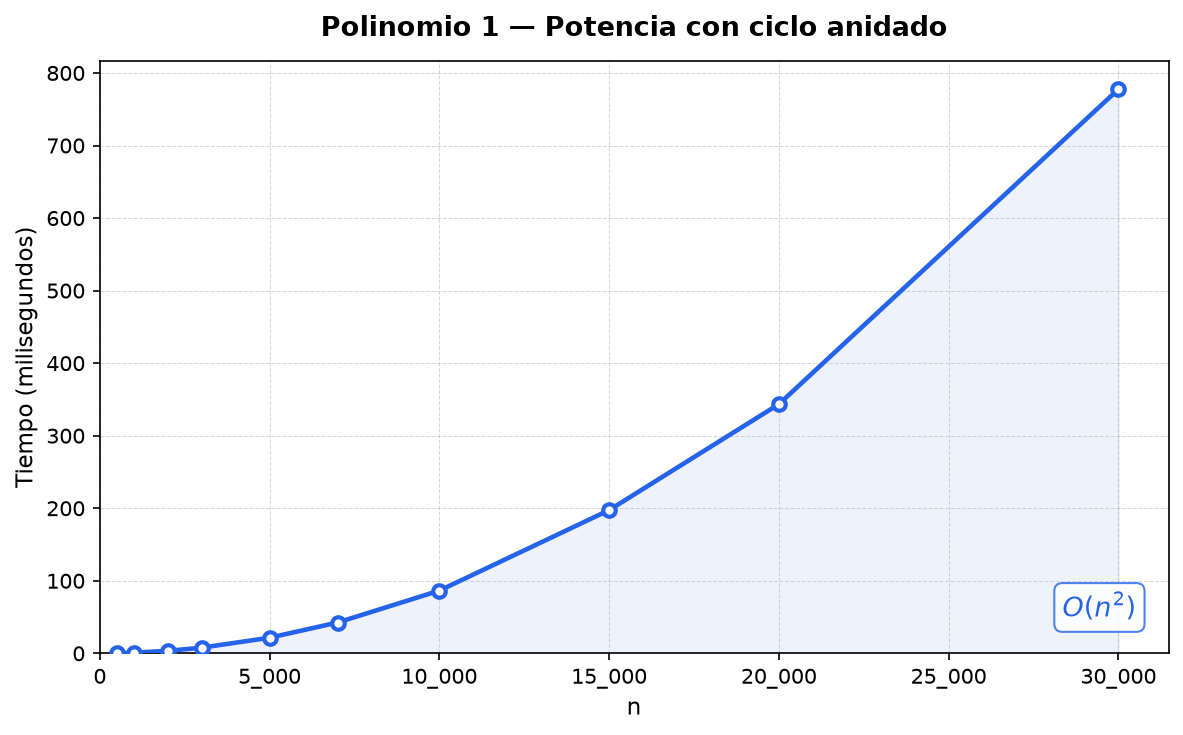
\includegraphics[width=0.8\textwidth]{../algoritmos/graphs/Polinomio1.png}
\end{figure}



% --------------------------------------------



\newpage
\subsection{Algoritmo 2 - Potencia recursiva}
\subsubsection{Código}
\begin{lstlisting}
double Potencia(double X, int j)
{
    if(j == 0)
    {
        return 1.0;
    }
    else if(j % 2 == 1)
    {
        return X * Potencia(X, j - 1);
    }
    else
    {
        double t = Potencia(X, j / 2);

        return t * t;
    }
}

double Polinomio2(const vector<double>& C, double X)
{
    int N = C.size() - 1;

    double S = C[0];

    for(int i = 0; i <= N; ++i)
    {
        S += C[i] * Potencia(X, i);
    }

    return S;
}
\end{lstlisting}


\subsubsection{Tiempos de ejecución}
\begin{table}[ht]
  \centering
  \begin{tabular}{rr}
    \toprule
    $n$ & Tiempo ($O(n \log n)$)\\
    \midrule
    10,000 & 857.8920\,µs \\
    50,000 & 5.4186\,ms \\
    100,000 & 12.2009\,ms \\
    500,000 & 71.8926\,ms \\
    1,000,000 & 155.4319\,ms \\
    2,000,000 & 333.4747\,ms \\
    3,000,000 & 518.5661\,ms \\
    5,000,000 & 909.9825\,ms \\
    7,000,000 & 1.2990\,s \\
    10,000,000 & 1.9221\,s \\
    \bottomrule
  \end{tabular}
\end{table}

\newpage
\subsubsection{Gráfica de tiempos}
\begin{figure}[!ht]
    \centering
    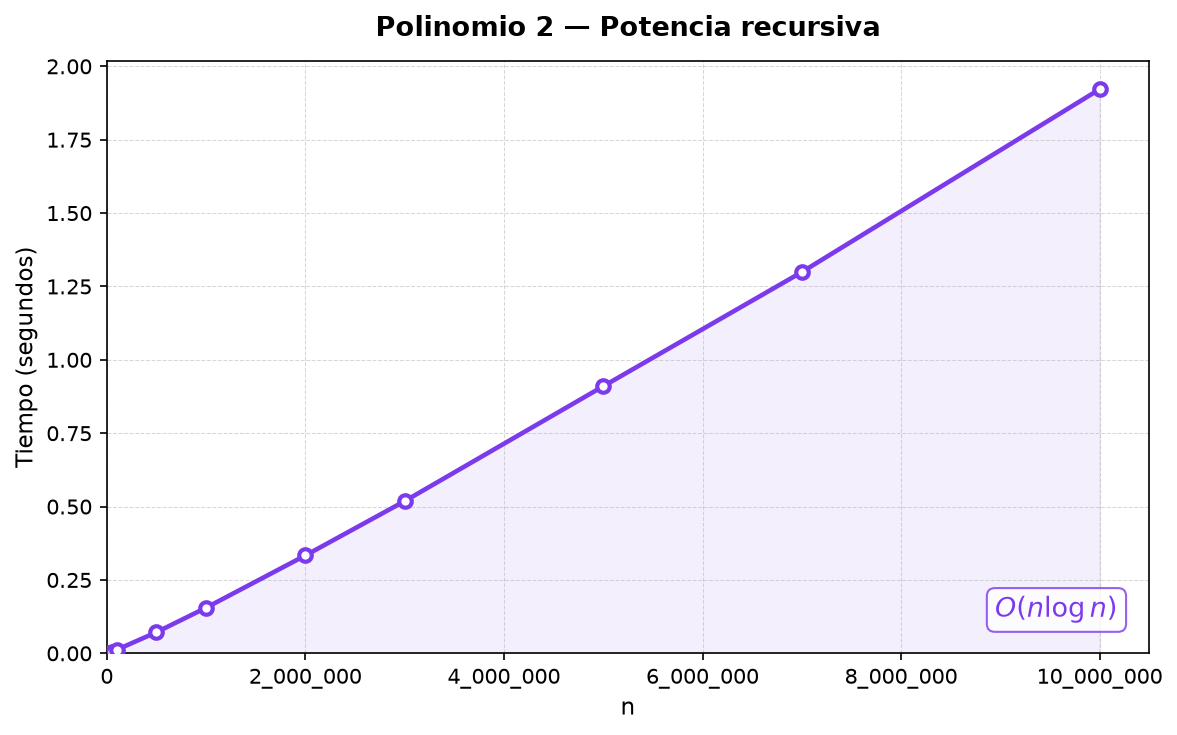
\includegraphics[width=0.8\textwidth]{../algoritmos/graphs/Polinomio2.png}
\end{figure}



% --------------------------------------------



\subsection{Algoritmo 3 - Multiplicación acumulada}
\subsubsection{Código}
\begin{lstlisting}
double Polinomio3(const vector<double>& C, double X)
{
    int N = C.size() - 1;

    double XN = 1.0;
    double S = C[0];

    for(int i = 0; i <= N; ++i)
    {
        XN *= X;
        S += C[i] * XN;
    }

    return S;
}
\end{lstlisting}

\newpage
\subsubsection{Tiempos de ejecución}
\begin{table}[ht]
  \centering
  \begin{tabular}{rr}
    \toprule
    $n$ & Tiempo ($O(n)$) \\
    \midrule
    10,000 & 20.4010\,µs \\
    50,000 & 101.5430\,µs \\
    100,000 & 202.8740\,µs \\
    500,000 & 1.0646\,ms \\
    1,000,000 & 2.1265\,ms \\
    2,000,000 & 4.1067\,ms \\
    3,000,000 & 6.6811\,ms \\
    5,000,000 & 10.3838\,ms \\
    7,000,000 & 15.6404\,ms \\
    10,000,000 & 22.8040\,ms \\
    \bottomrule
  \end{tabular}
\end{table}

\subsubsection{Gráfica de tiempos}
\begin{figure}[!ht]
    \centering
    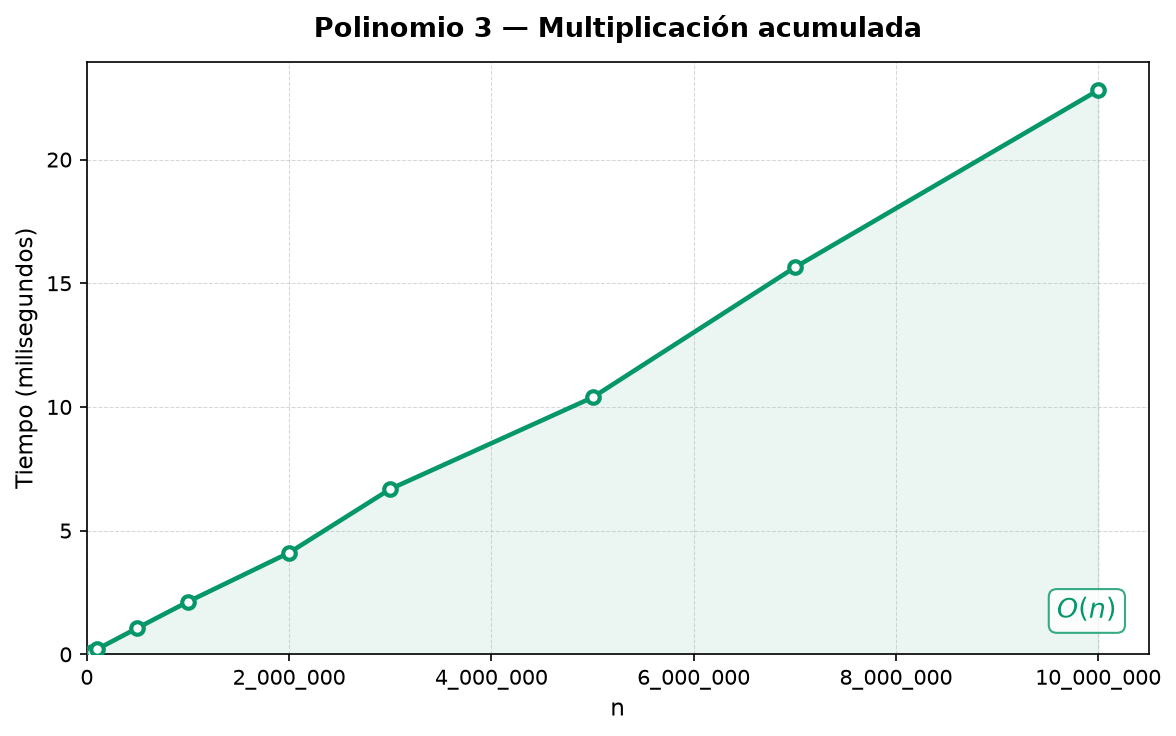
\includegraphics[width=0.8\textwidth]{../algoritmos/graphs/Polinomio3.png}
\end{figure}



% --------------------------------------------



\subsection{Algoritmo 4 - Regla de Horner}
\subsubsection{Código}
\begin{lstlisting}
double Polinomio4(const vector<double>& C, double X)
{
    int N = C.size() - 1;
    double S = 0.0;

    for(int i = N; i >= 0; --i)
    {
        S = S * X + C[i];
    }

    return S;
}
\end{lstlisting}


\subsubsection{Tiempos de ejecución}
\begin{table}[ht]
  \centering
  \begin{tabular}{rr}
    \toprule
    $n$ & Tiempo ($O(n)$) \\
    \midrule
    10,000 & 32.3010\,µs \\
    50,000 & 161.2660\,µs \\
    100,000 & 362.0410\,µs \\
    500,000 & 1.6219\,ms \\
    1,000,000 & 3.2598\,ms \\
    2,000,000 & 6.7007\,ms \\
    3,000,000 & 9.8165\,ms \\
    5,000,000 & 16.9991\,ms \\
    7,000,000 & 23.1858\,ms \\
    10,000,000 & 32.9864\,ms \\
    \bottomrule
  \end{tabular}
\end{table}

\subsubsection{Gráfica de tiempos}
\begin{figure}[!ht]
    \centering
    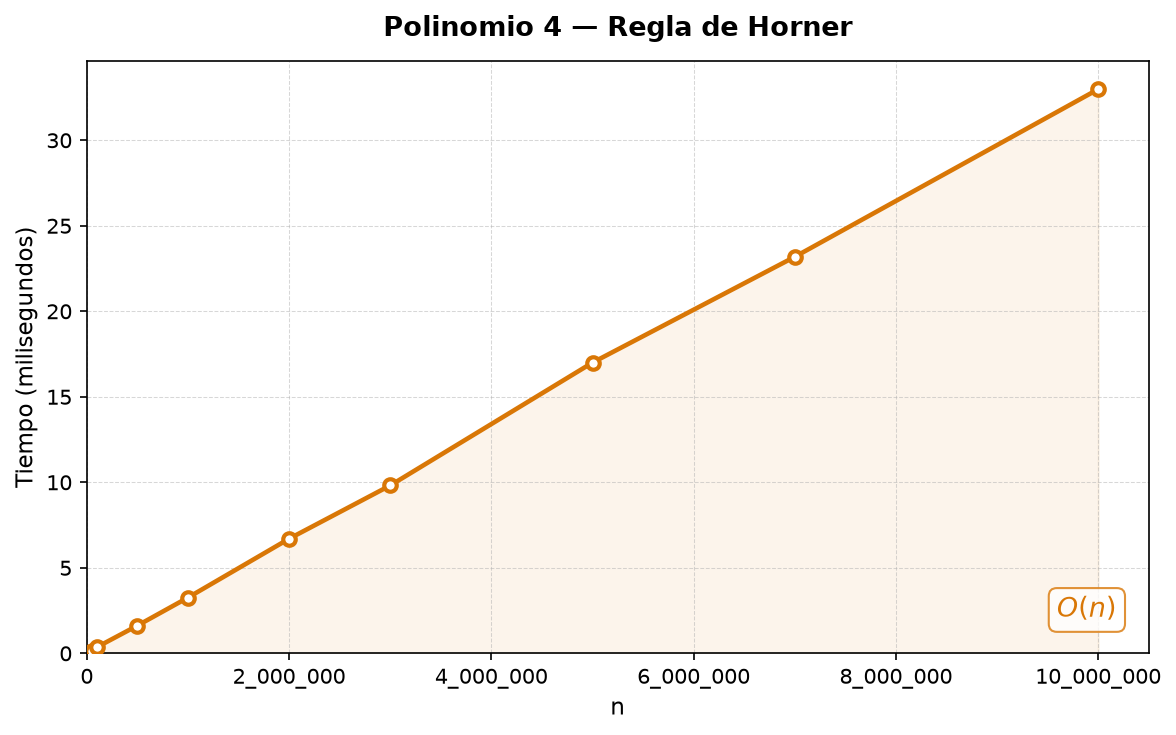
\includegraphics[width=0.8\textwidth]{../algoritmos/graphs/Polinomio4.png}
\end{figure}



% --------------------------------------------



\section{Sum}
\subsection{Código}
\begin{lstlisting}
float Sum(vector<float> a, int n)
{
    float s = 0.0;

    for(int i = 0; i < n; ++i) s += a[i];
    
    return s;
}
\end{lstlisting}

\newpage
\subsection{Tiempos de ejecución}
\begin{table}[ht]
  \centering
  \begin{tabular}{rr}
    \toprule
    $n$ & Tiempo ($O(n)$) \\
    \midrule
    100,000 & 218.7250\,µs \\
    500,000 & 1.0313\,ms \\
    1,000,000 & 2.1191\,ms \\
    2,000,000 & 4.5373\,ms \\
    3,000,000 & 6.4210\,ms \\
    5,000,000 & 13.4520\,ms \\
    7,000,000 & 20.7139\,ms \\
    10,000,000 & 32.6061\,ms \\
    15,000,000 & 50.9609\,ms \\
    20,000,000 & 66.9751\,ms \\
    \bottomrule
  \end{tabular}
\end{table}

\subsection{Gráfica de tiempos}
\begin{figure}[!ht]
    \centering
    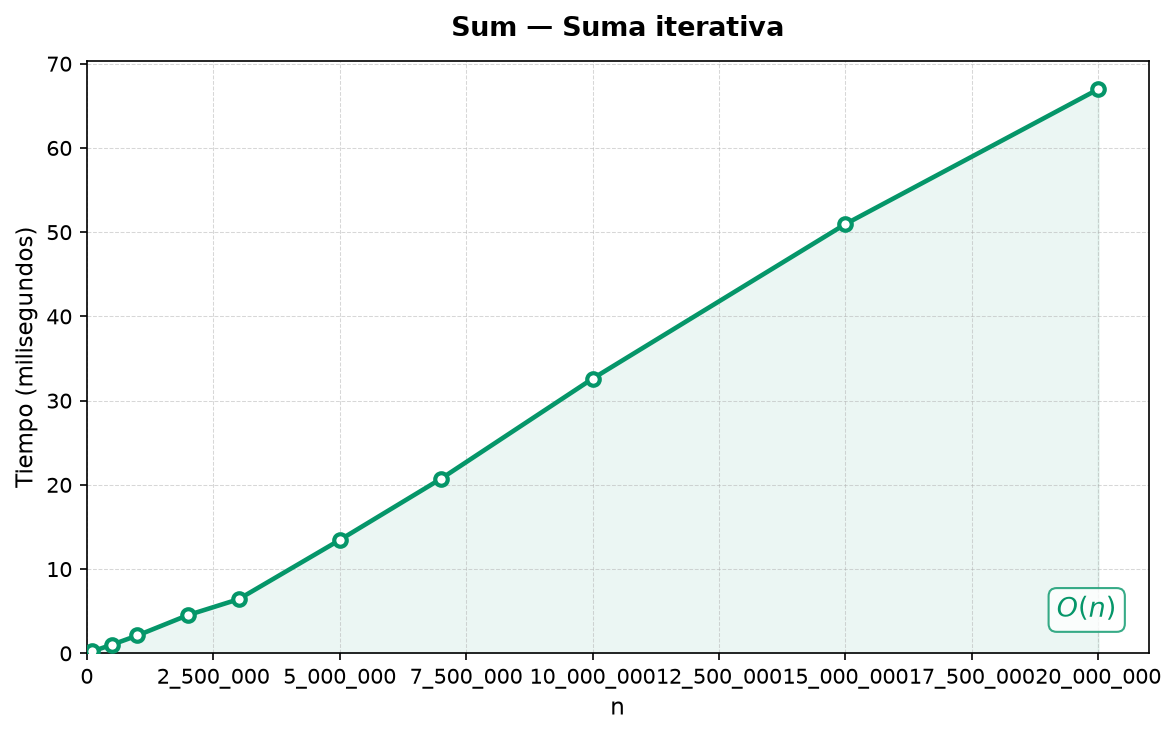
\includegraphics[width=0.8\textwidth]{../algoritmos/graphs/Sum.png}
\end{figure}



% --------------------------------------------



\newpage
\section{RSum}
\subsection{Código}
\begin{lstlisting}
float RSum(vector<float> a, int n)
{
    float result;
    if(n <= 0)
    {
        result = 0.0;
    }
    else
    {
        result = RSum(a, n - 1) + a[n-1];
    }

    return result;
}
\end{lstlisting}


\subsection{Tiempos de ejecución}
\begin{table}[ht]
  \centering
  \begin{tabular}{rr}
    \toprule
    $n$ & Tiempo ($O(n)$) \\
    \midrule
    1,000 & 335.7120\,µs \\
    2,000 & 1.0722\,ms \\
    3,000 & 2.1842\,ms \\
    5,000 & 19.0461\,ms \\
    7,000 & 44.3347\,ms \\
    10,000 & 137.0227\,ms \\
    12,000 & 182.7842\,ms \\
    15,000 & 289.1696\,ms \\
    18,000 & 408.5071\,ms \\
    20,000 & 577.4380\,ms \\
    \bottomrule
  \end{tabular}
\end{table}

\subsection{Gráfica de tiempos}
\begin{figure}[!ht]
    \centering
    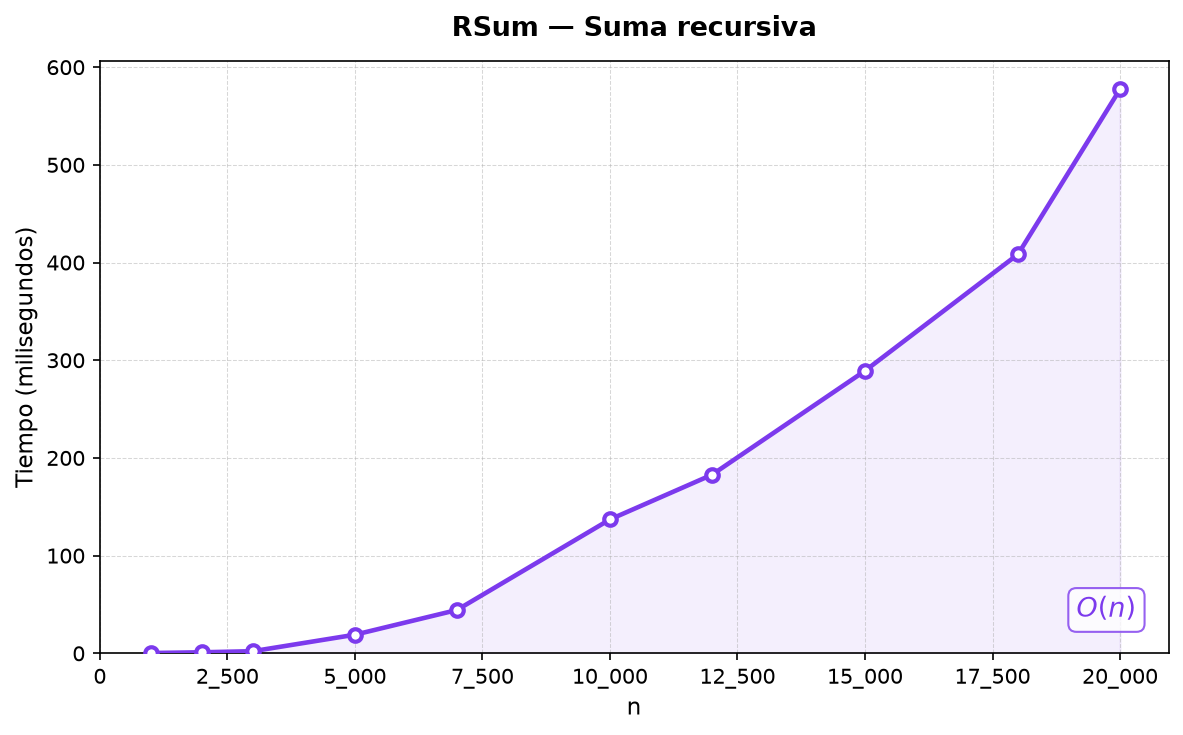
\includegraphics[width=0.7\textwidth]{../algoritmos/graphs/RSum.png}
\end{figure}



% --------------------------------------------



\section{Add}
\subsection{Código}
\begin{lstlisting}
vector<vector<float>> Add(vector<vector<float>> a, vector<vector<float>> b, int n)
{
    vector<vector<float>> c(n, vector<float>(n));

    for(int i = 0; i < n; ++i)
    {
        for(int j = 0; j < n; ++j)
        {
            c[i][j] = a[i][j] + b[i][j];
        }
    }
    return c;
}
\end{lstlisting}


\subsection{Tiempos de ejecución}
\begin{table}[ht]
  \centering
  \begin{tabular}{rr}
    \toprule
    $n$ & Tiempo ($O(n^2)$) \\
    \midrule
    100 & 165.8420\,µs \\
    200 & 557.6420\,µs \\
    400 & 2.2490\,ms \\
    600 & 5.2358\,ms \\
    800 & 8.8062\,ms \\
    1,000 & 13.6477\,ms \\
    1,200 & 20.1402\,ms \\
    1,500 & 33.1476\,ms \\
    1,800 & 48.9597\,ms \\
    2,000 & 67.0839\,ms \\
    \bottomrule
  \end{tabular}
\end{table}

\subsection{Gráfica de tiempos}
\begin{figure}[!ht]
    \centering
    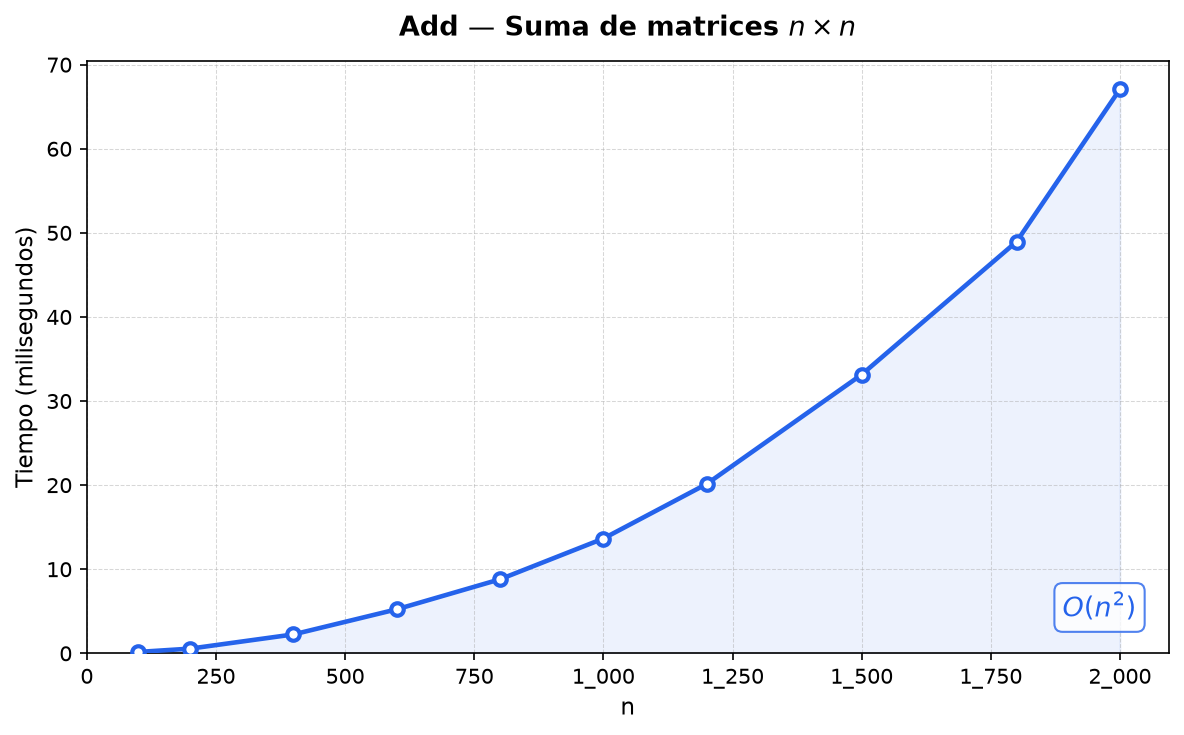
\includegraphics[width=0.7\textwidth]{../algoritmos/graphs/Add.png}
\end{figure}



% --------------------------------------------



\section{Trasp}
\subsection{Código}
\begin{lstlisting}
void Trasp(vector<vector<float>> & a, int n)
{
    float t = 0.0;

    for(int i = 0; i < n-1; ++i)
    {
        for(int j = i+1; j < n; ++j)
        {
            t = a[i][j];
            a[i][j] = a[j][i];
            a[j][i] = t;
        }
    }
}
\end{lstlisting}


\subsection{Tiempos de ejecución}
\begin{table}[ht]
  \centering
  \begin{tabular}{rr}
    \toprule
    $n$ & Tiempo ($O(n^2)$) \\
    \midrule
    100 & 41.5410\,µs \\
    300 & 372.5950\,µs \\
    600 & 1.4871\,ms \\
    900 & 3.3472\,ms \\
    1,200 & 6.3003\,ms \\
    1,500 & 9.9603\,ms \\
    2,000 & 17.7941\,ms \\
    2,500 & 29.3245\,ms \\
    3,500 & 59.3193\,ms \\
    5,000 & 155.1489\,ms \\
    \bottomrule
  \end{tabular}
\end{table}

\subsection{Gráfica de tiempos}
\begin{figure}[!ht]
    \centering
    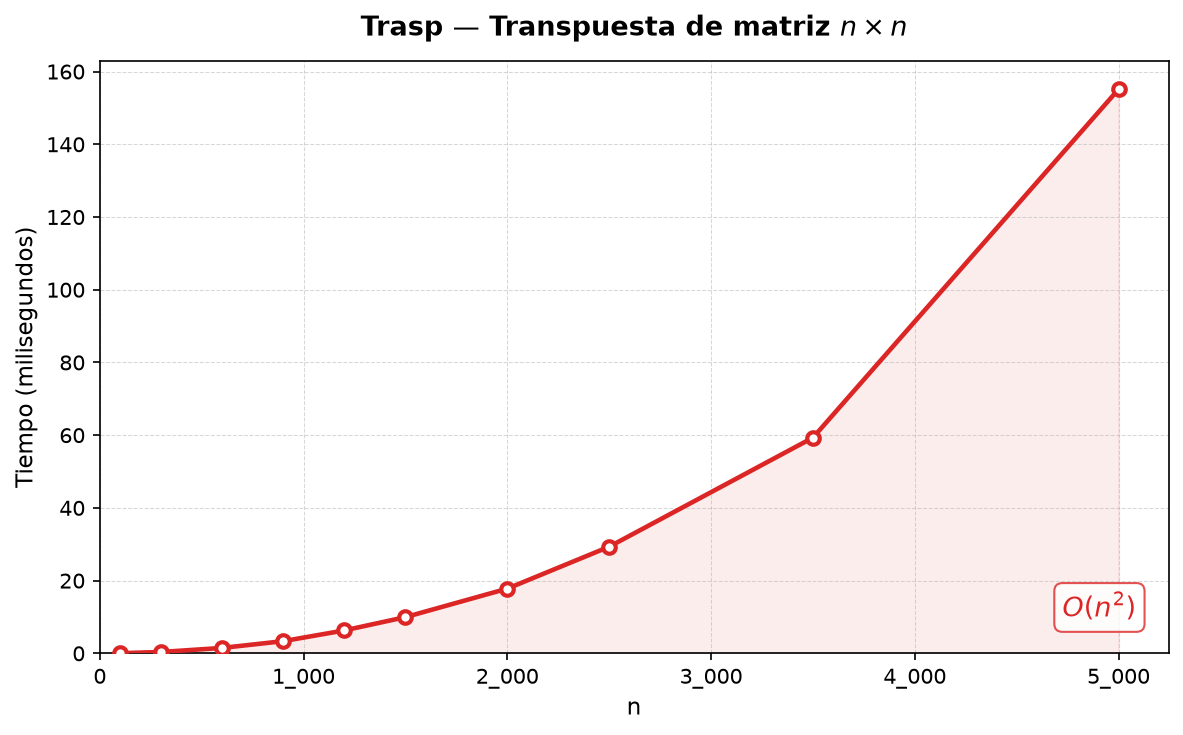
\includegraphics[width=0.7\textwidth]{../algoritmos/graphs/Trasp.png}
\end{figure}



% --------------------------------------------



\section{Mult}
\subsection{Código}
\begin{lstlisting}
vector<vector<float>> Mult(const vector<vector<float>>& a, const vector<vector<float>>& b)
{
    int n = a.size();

    vector<vector<float>> c(n, vector<float>(n, 0.0f));

    for(int i = 0; i < n; ++i)
    {
        for(int j = 0; j < n; ++j)
        {
            for(int k = 0; k < n; ++k)
            {
                c[i][j] += a[i][k] * b[k][j];
            }
        }
    }

    return c;
}
\end{lstlisting}


\subsection{Tiempos de ejecución}
\begin{table}[ht]
  \centering
  \begin{tabular}{rr}
    \toprule
    $n$ & Tiempo ($O(n^3)$) \\
    \midrule
    100 & 12.7125\,ms \\
    200 & 100.1668\,ms \\
    300 & 325.6764\,ms \\
    400 & 768.2177\,ms \\
    500 & 1.5144\,s \\
    600 & 2.6010\,s \\
    700 & 4.1743\,s \\
    800 & 6.2492\,s \\
    900 & 8.9168\,s \\
    1,000 & 12.2373\,s \\
    \bottomrule
  \end{tabular}
\end{table}

\newpage
\subsection{Gráfica de tiempos}
\begin{figure}[!ht]
    \centering
    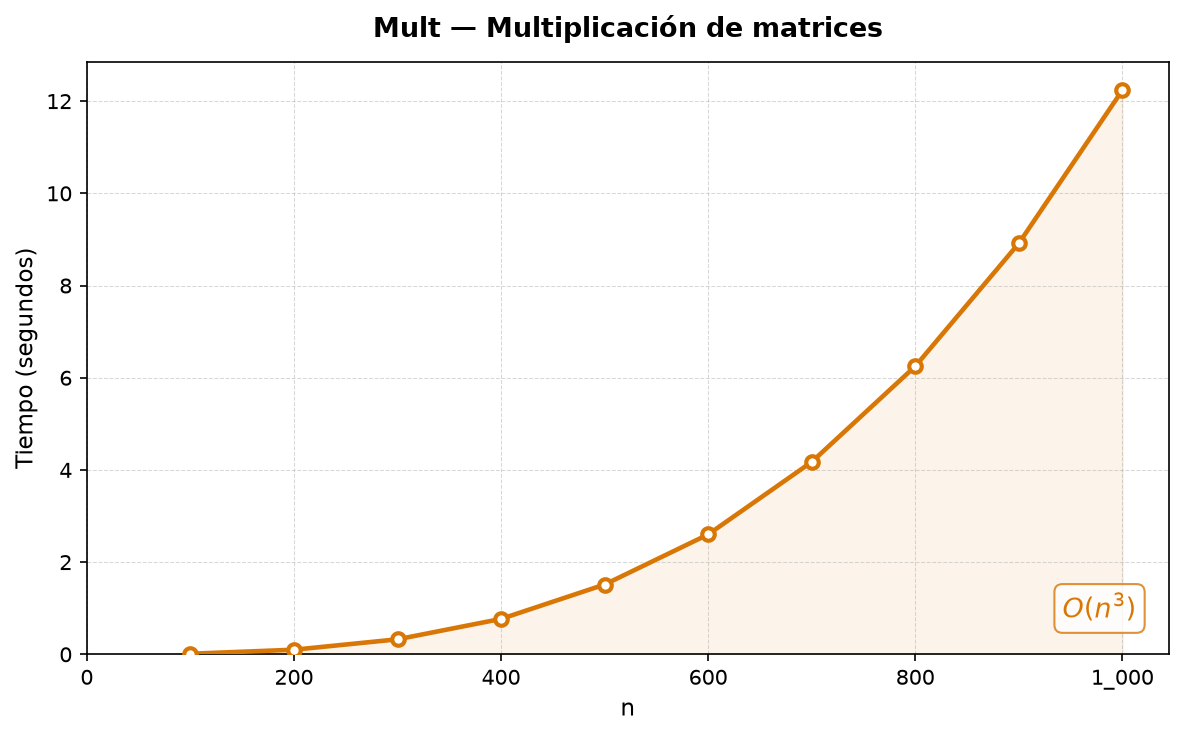
\includegraphics[width=0.8\textwidth]{../algoritmos/graphs/Mult.png}
\end{figure}



% --------------------------------------------



\section{Perm}
\subsection{Código}
\begin{lstlisting}
void Perm(vector<int>& a, int k, int n)
{
    if(k == n)
    {
        for(int i = 0; i < n; ++i)
        {
            cout << a[i] << " ";
        }
        cout << endl;
    }
    else
    {
        for(int i = k; i < n; ++i)
        {
            swap(a[k], a[i]);

            Perm(a, k + 1, n);

            swap(a[k], a[i]);
        }
    }
}
\end{lstlisting}

\newpage
\subsection{Tiempos de ejecución}
\begin{table}[ht]
  \centering
  \begin{tabular}{rr}
    \toprule
    $n$ & Tiempo ($O(n!)$) \\
    \midrule
    3 & 422\,ns \\
    4 & 1.1730\,µs \\
    5 & 5.3820\,µs \\
    6 & 25.0260\,µs \\
    7 & 174.0150\,µs \\
    8 & 1.4394\,ms \\
    9 & 13.4568\,ms \\
    10 & 127.1139\,ms \\
    11 & 1.3867\,s \\
    12 & 16.6943\,s \\
    \bottomrule
  \end{tabular}
\end{table}

\subsection{Gráfica de tiempos}
\begin{figure}[!ht]
    \centering
    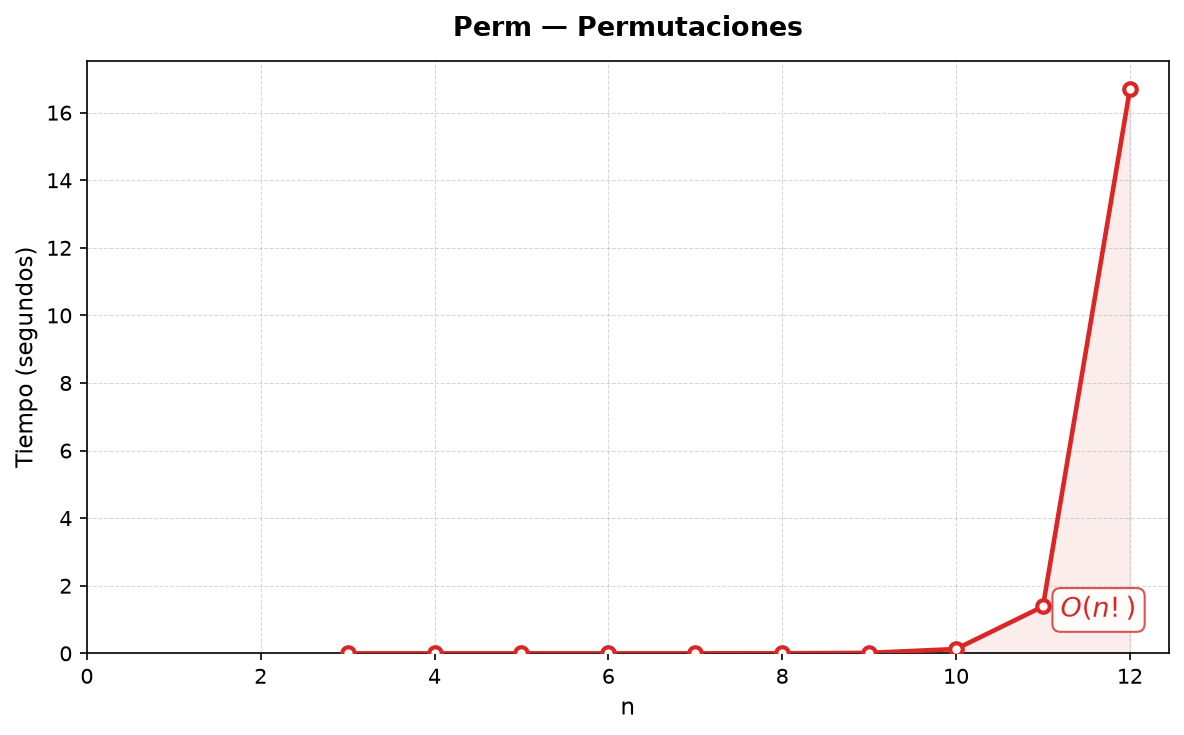
\includegraphics[width=0.8\textwidth]{../algoritmos/graphs/Perm.png}
\end{figure}



% --------------------------------------------



\newpage
\section{SeqSearch}
\subsection{Código}
\begin{lstlisting}
int SeqSearch(vector<int>& a, int x)
{
    int n = a.size() - 1;
    a[0] = x;
    int i = n;

    while(a[i] != x)
    {
        i = i - 1;
    }
    return i;
}
\end{lstlisting}


\subsection{Tiempos de ejecución}
\begin{table}[ht]
  \centering
  \begin{tabular}{rr}
    \toprule
    $n$ & Tiempo ($O(n)$) \\
    \midrule
    100,000 & 179.0700\,µs \\
    500,000 & 895.7680\,µs \\
    1,000,000 & 1.7590\,ms \\
    5,000,000 & 9.3681\,ms \\
    10,000,000 & 17.6167\,ms \\
    20,000,000 & 36.9621\,ms \\
    30,000,000 & 53.1168\,ms \\
    50,000,000 & 90.5206\,ms \\
    75,000,000 & 137.4871\,ms \\
    100,000,000 & 177.4072\,ms \\
    \bottomrule
  \end{tabular}
\end{table}

\subsection{Gráfica de tiempos}
\begin{figure}[!ht]
    \centering
    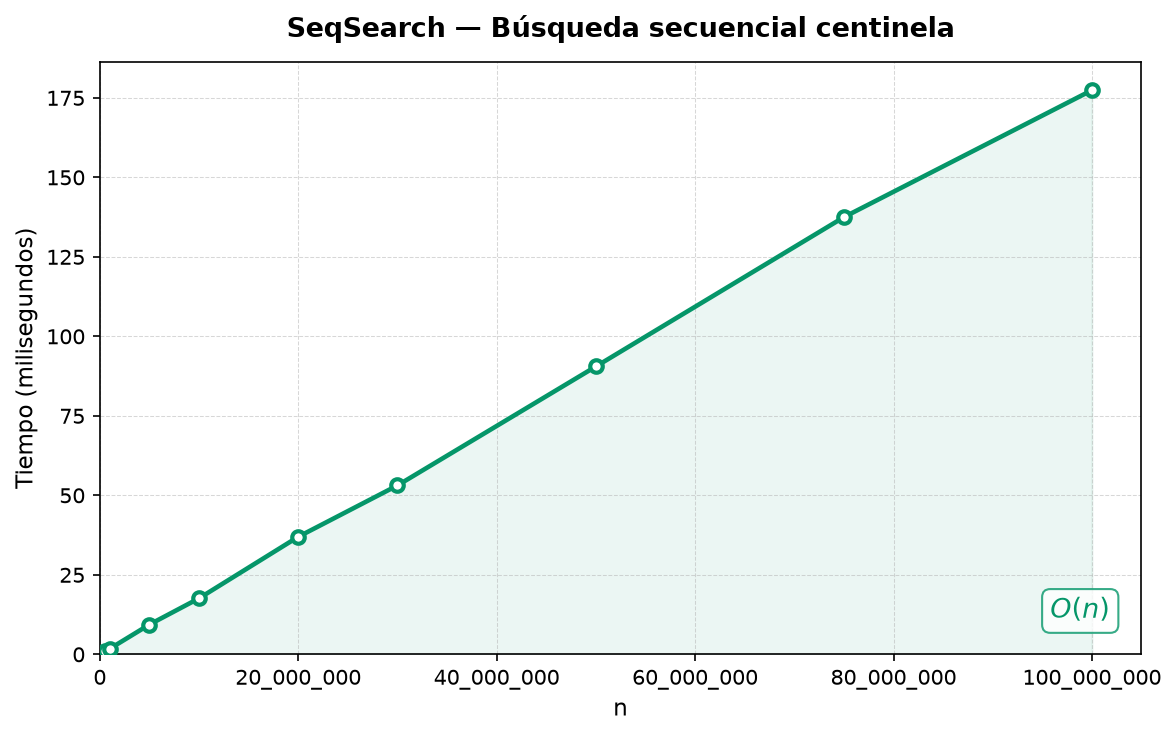
\includegraphics[width=0.7\textwidth]{../algoritmos/graphs/SeqSearch.png}
\end{figure}
\end{document}
